% Chapter 4

\chapter{A Deep LSTM Network for Short Term Traffic Prediction} % Main chapter title

\label{Chapter4} % For referencing the chapter elsewhere, use \ref{Chapter4}

% This is for the header on each page - perhaps a shortened title
\lhead{Chapter 4. \emph{A Deep LSTM Network for Short Term Traffic Prediction}}

% Quotation
{``I am a brain, Watson. The rest of me is a mere appendix."}
\begin{flushright}
Arthur Conan Doyle, \textit{The Adventure of the Mazarin Stone} (1921)
\end{flushright}

%---------------------------------------------------------------------------------------------------
%	CONTENT
%  \cite{bengio2015deep,graves2013generating,hochreiter2001gradient,bengio1994learning,
%       gers2000learning,hochreiter1997long}
%  \cite{busseti2012deep} \cite{karpathy2015visualizing} \cite{graves2012supervised}
% \cite{bishop2007pattern} \cite{gers2001long}
%---------------------------------------------------------------------------------------------------

In section \ref{subsec:neuralNetworksTrafficPred}, we presented a brief introduction to artificial
neural networks and reviewed existing literature in short term traffic prediction that used
various types of neural networks. In the following sections we present a bried overview of deep
learning. We then describe deep feedforward networks, deep recurrent networks with emphasis on
the Long Short Term Memory(LSTM) networks which are a redesigned version of recurrent networks.
Later we present how we can we can use these kind of networks for short term traffic prediction.

\section{Introduction}
Today we live in a world where almost every interaction of ours with the external world uses some
form of computing. Computers have become an inseparable part of human lives. In the earlier days
when computers were built, people began to ponder whether they could achieve human level
of intelligence. Even though at that point the answers seemed optimistic, it has taken quite
some time and understanding on our part to make significant achievements in the field of
artificial intelligence. One of the approaches was to use knowldge base systems, where computers
reason about real world concepts, that were defined in hard-coded formal langauges, using logical
inference rules. These systems led to little success. The difficulties faced in the knwoledge
based appproach made us built computers to learn automatically from data, an approach we know as
machine learning.

A large number of real world problems could eaily be tackled using machine leraning. However for
the machine learning algorithms to perorm well they need to be provided with proper representaion
of data. For example, in a problem where we would like to detect humans in images, it is
difficult to represent various shapes of human body in terms of raw pixels. Finding a proper
representation from data is a challenge and sometimes become very difficult. A class of machine
learning algorithms called representation learning, tackles this problem by learning the
representaions as well. Autoencodes are such types of algorithms. Again the problem with
representation learing is that it is not easy to find the representations due to the presence of
various factors of influence (\citet{bengio2015deep}). Deep learning solves this problem in
representation learning by taking a layered approach by expressing representations in terms of
simpler representations. The mapping from the input to output is done through a series of hidden
layers, where each layer is an abstraction on the previous layer. The depth of the model can be
viewed as the depth of the computational graph, i.e. the number of sequential instructions that
need to be executed to map an input to output.

\section{Feedforward neural networks}
Deep feedforward networks are the most important deep learning models. The main goal of a deep
feedforward network is to approximate a function $f^{*}$ that maps an input $\textbf{x}$ to an
output $y$. As the name implies, the information in these models flow in the forward direction.
These are the basis of several models used in commercial applications such as the convolutional
networks, which are extensions of the feedforward networks, have been very successful in image
recognition. With the addition of feedback connections to feedforward networks, recurrent
networks are created. Feedforward networks consist of a chain of layers, which is simply done by
composing functions for instance we can compose three functions as to map an input $\textbf{x}$
to an output $y$, $y = f(\textbf{x}) = f^{3}(f^{2}(f^{1}))$. Function $f^{2}$ acts as the hidden
layer that maps the output from the input layer $f^{1}$ to the input of the output layer $f^{3}$.

The diagram \ref{fig:ffnnetwork} illustrates a simple feedforward neural network with 3 nodes in
the input layer, 3 and 4 nodes in two hidden layers and a single node output layer. Information
propagates from the input layer through the hidden layer to the output layer, known as the
forward pass of the network. This kind of feedforward network is called a multilayer perceptron.
Multilayer perceptrons are good at classification.

    \def\layersep{2.5cm}
    \begin{figure}
    \centering
    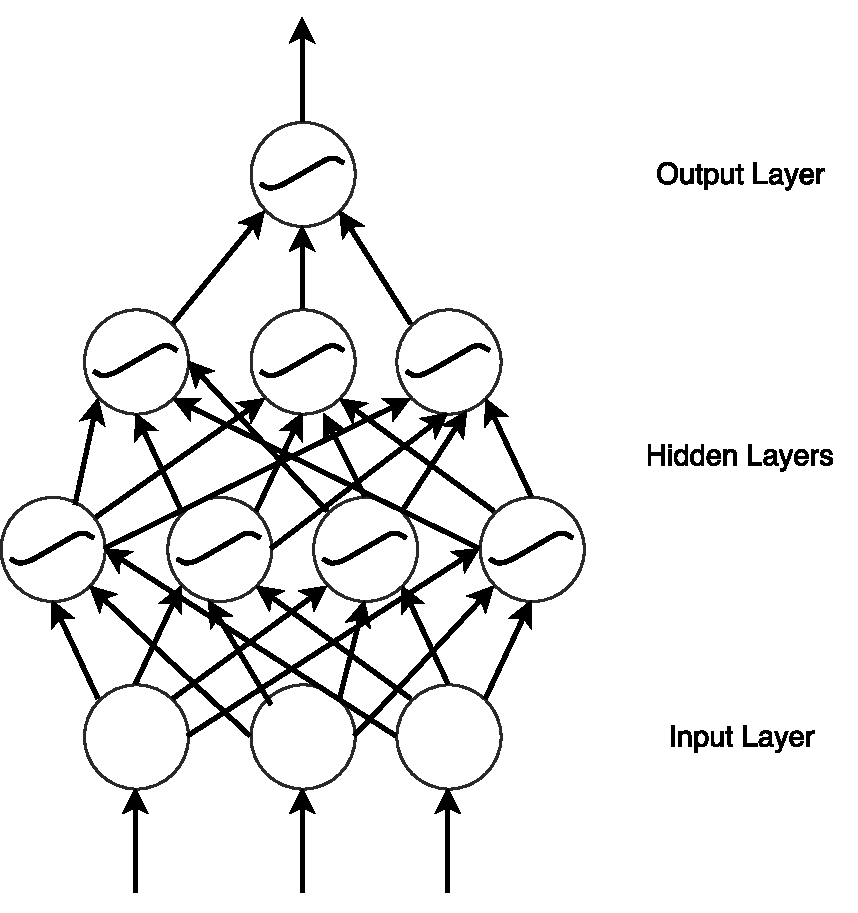
\includegraphics[width=\textwidth,height=0.5\textheight,keepaspectratio]
        {Figures/mlp.pdf}
        \rule{35em}{0.5pt}
    \caption[Multilayer perceptron]
    {A feedforward neural netwrok with two hidden layers, this network is also known as a
    multilayer perceptron. The S-shaped curves denote the sigmoidal function.}
    \label{fig:ffnnetwork}
    \end{figure}

Let's consider a simple multilayer perceptron with \textit{I} nodes in the input layer. For an
input vector \textbf{x}, where length of \textbf{x} is \textit{I}. Each node in
the hidden layer gets a weighted sum of the units in the input layer. The output of each hidden unit
$a_{h}$ is then applied to an activation function $\theta_{h}$ to produce the activation $b_{h}$

    \begin{equation}
        a_{h} = \displaystyle\sum_{i=1}^\textit{I} w_{ih}x_{i}
    \end{equation}

    \begin{equation}
        b_{h} = \theta_{h}(a_{h})
    \end{equation}

There are several choices for the activation functions with sigmoidal and hyperbolic tan
fucntions are the most common choices. The reason of these choices is nonlinearity of
these functions. Recently the recommended activation function for feedforward neural networks is
the \emph{rectified linear unit} or ReLU (\citet{nair2010rectified}), defined as $f(x) = max{0,x}$,
as they allow faster and efficient training of deep neural network architectures.

The activations flow through the rest of the hidden layers in similar fashion. For instance the
$l^{th}$ hidden unit in layer $H_{l}$
    \begin{equation}
        a_{h} = \displaystyle\sum_{h' \in H_{l-1}} w_{h'h}b_{h'}
    \end{equation}

    \begin{equation}
        b_{h} = \theta_{h}(a_{h})
    \end{equation}

In the output layer, the activation function is applied on the output from the hidden layer to
produce the output y. The input $a_{k}$ to the output unit is given by

    \begin{equation}
        a_{k} = \displaystyle\sum_{h \in H_{L}} w_{hk}b_{h}
    \end{equation}

where L is the number of hidden layers in the network. The number of units in the output layer
and the type of activation function are chosen based on the problem task at hand. For binary
classification a single unit with logistic sigmoid activation function is primarily used. For
classification with k > 2 classes, k output units are used and the outputs are normalised using
the \emph{softmax} function. A very common example of this is the hand-written digits classification,
where the output layer consists of 10 units.

\section{Recurrent neural networks}
As mentioned earlier, we can create a recurrent neural network by adding feedback connections to
a feedforward network. Several types of recurrent neural networks have been proposed over the
years, some of which are - \emph{echo state networks, time delay networks, jordan networks}. At
first the difference between a feedforward and a recurrent network may not be obvious and seem
trvial but recurrent networks are very powerful in the sense that they can retain the history and
thus forming a memory in their feedback connections.

\begin{figure}[htbp]
  \centering
    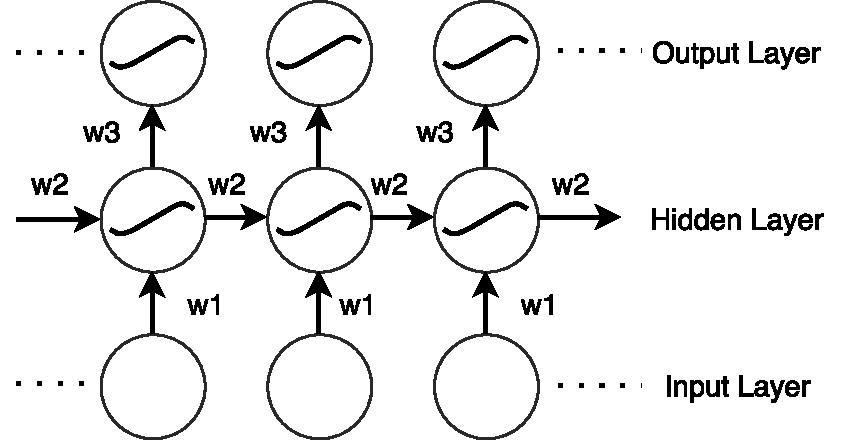
\includegraphics[width=\textwidth,height=\textheight,keepaspectratio]
    {Figures/unfolded-rnn.pdf}
    \rule{35em}{0.5pt}
  \caption[An unfolded RNN] {An unfolded recurrent neural network. w1, w2 and w3 are weighted
  connections. }
  \label{fig:unfoldedRNN}
\end{figure}

\section {Network training using gradient descent}
Training neural networks is no different than any other machine learning models with a loss
function and gradient descent algorithm. However the difficulty is that the non-linear
characteristics of neural networks causes to the loss functions to become non-convex. So the
training procedure usually involves small iterative gradient descent algorithm to get a very low
value of the cost function. For feedforward networks the weights are initialised with very small
random numbers and the biased may be initilised to zero or very small values as well.

The choice of a cost function is somehow important and usually these are same as the linear models.

\section{LSTM networks}
In previous section we learn that using a recurrent neural networks we can store information in
form of activations in the feedback connnections. The major disadvantage with recurrent neural
networks is their inability to ratain information for a long period of time. This is caused by an
effect known as \emph{vanishing gradient problem}(\citet{bengio1994learning},
\citet{hochreiter2001gradient}). The vanishing gradient problem is depicted in the figure
\ref{fig:vanishingGradient}. Number of attempts were made in the 1990's to resolve this issue.
\citet{hochreiter1997long} proposed a redesigned network called Long Short Term Momory(LSTM) to
address this problem.

\begin{figure}[htbp]
  \centering
    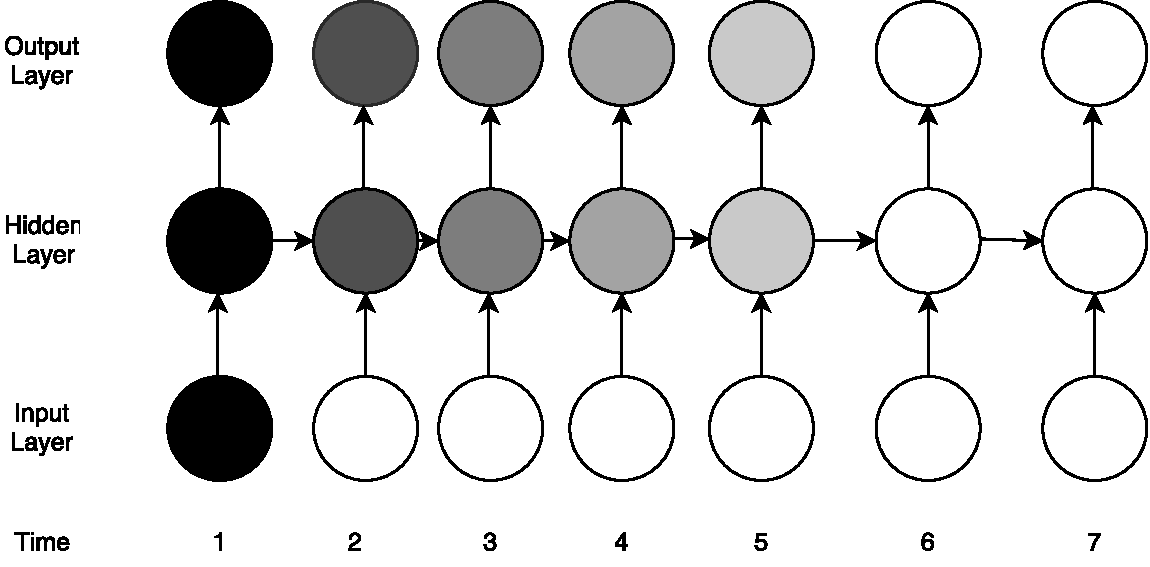
\includegraphics[width=\textwidth,height=\textheight,keepaspectratio]{Figures/vanishing-gradient.pdf}
    \rule{35em}{0.5pt}
  \caption[Vanishing Gradient] {The problem of vanishing gradient in recurrent neural networks.
  The sensitivity, as indicated by the shading, gradually diminishes with time}
  \label{fig:vanishingGradient}
\end{figure}


\subsection{Architecture}
An LSTM network is a set of recurrently connected LSTM blocks, also known as memory blocks, where
each memory block has one or more memory cells and three units (input, output and forget gates)
that perform the read, write and reset operations. A basic LSTM block with one memory cell is
depicted in the figure \ref{fig:lstmBlock}. The multiplicative units allow the LSTM to store
information for a long time and thus addresses the problem of vanishing gradient. An LSTM network
is shown in figure \ref{fig:lstmNetwork}, the hidden layers contains the LSTM blocks.

\begin{figure}[htbp]
  \centering
    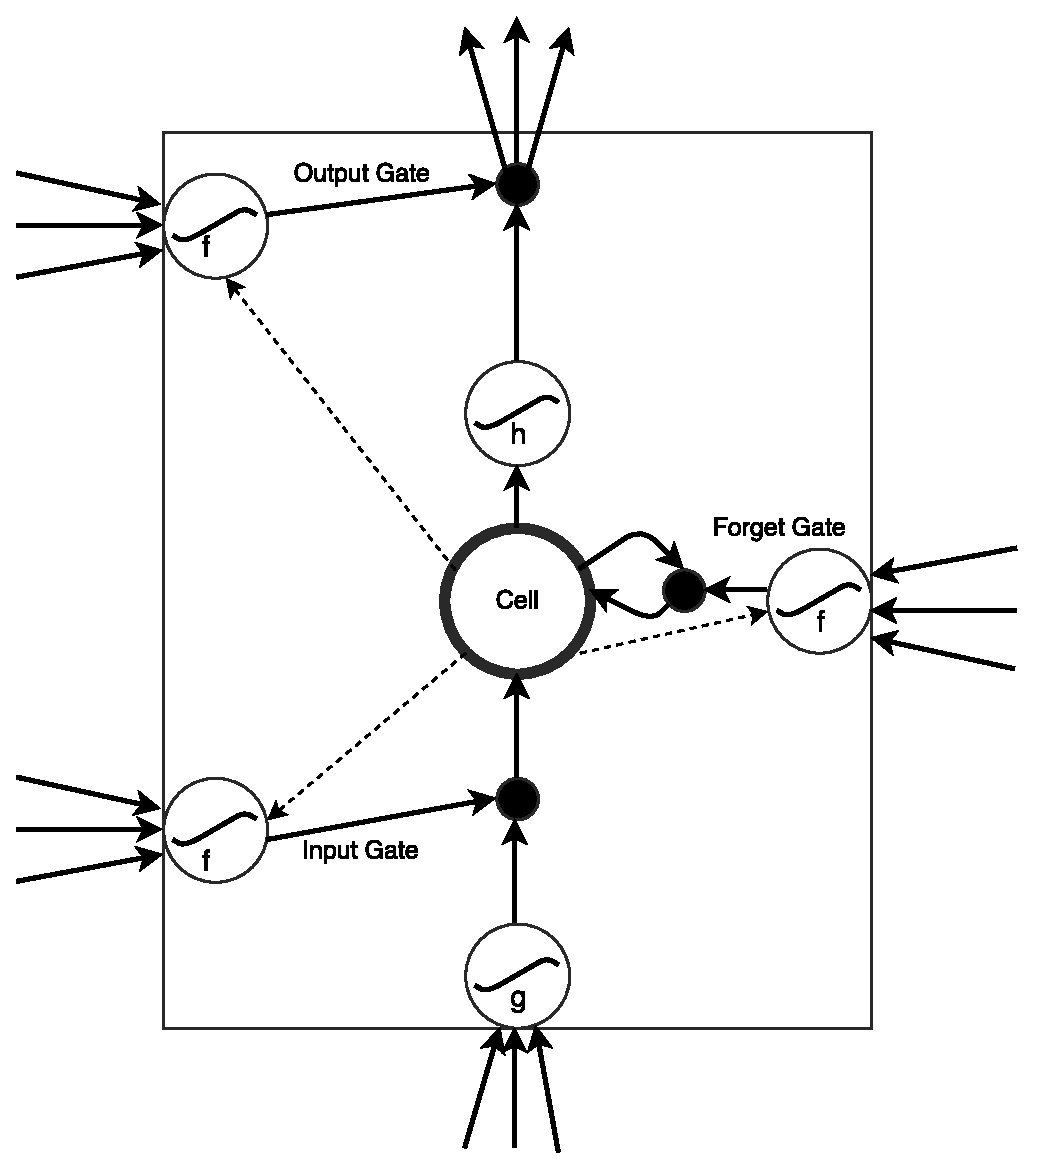
\includegraphics[width=\textwidth,height=0.5\textheight,keepaspectratio]{Figures/lstm-block.pdf}
    \rule{35em}{0.5pt}
  \caption[An LSTM block with one cell]
{An LSTM block with one cell. The three units collect activations from both inside and outside of
the block. The small black circles represents mulitipications by which the gates control the
memory cell. The gate activation function is f, usually a logistic sigmoid. The cell input and
output functions are g and h, usually tanh or logistic sigmoid. The dashed lines represent the
weighted peephole connections from the cell to the gates. All other connections are not weighted.
The only outputs from the block to the rest of the network is from the output gate multiplication.}
  \label{fig:lstmBlock}
\end{figure}

\begin{figure}[htbp]
  \centering
    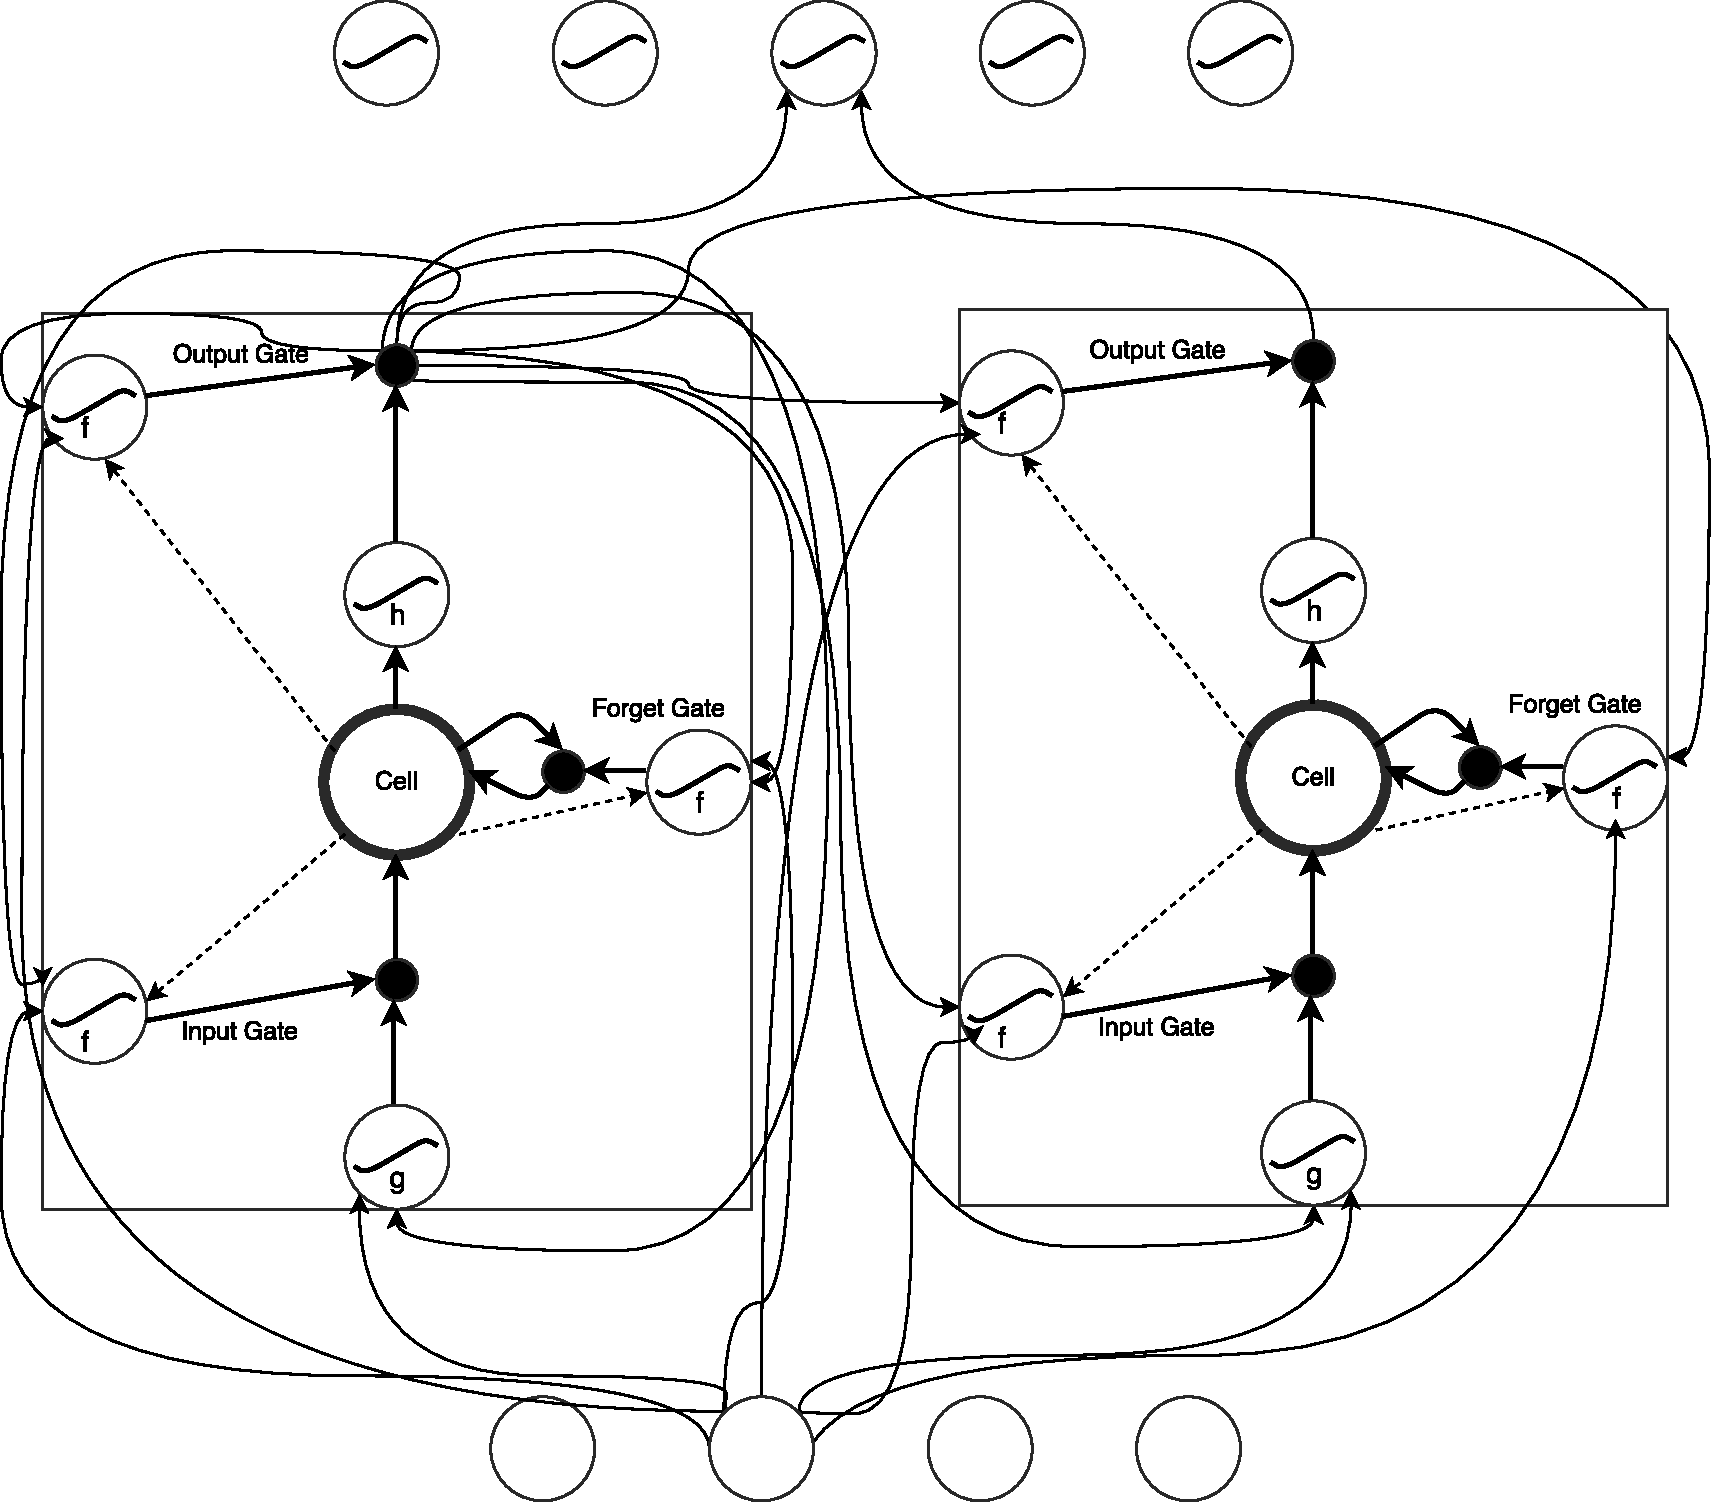
\includegraphics[width=\textwidth,height=\textheight,keepaspectratio]{Figures/lstm-network.pdf}
    \rule{35em}{0.5pt}
  \caption[An LSTM network]
{An LSTM network with one hidden layer with two memory blocks. The input layer consists of
four input units and the output layer consists of five output units. Not all connections are
shown in the figure. There is only one output from the block.}
  \label{fig:lstmNetwork}
\end{figure}

\subsection{Training}

\section{A Stacked LSTM network for short term traffic prediction}
\label{sec:stackedLSTMTrafficPred}

